\documentclass{article}
\usepackage[%
    left=0.5in,%
    right=0.5in,%
    top=0.5in,%
    bottom=0.5in,%
]{geometry}%
\usepackage{minitoc}
\usepackage{multicol}
\usepackage{graphicx}
\usepackage{fixltx2e}
\usepackage{hyperref}
\usepackage{hyperref}
    \hypersetup{ colorlinks = true, linkcolor = blue }
\usepackage{blindtext}

\graphicspath{ {./} }

\newcommand{\worddef}[1]{\hyperref[sec:reference]{\textit{#1}}}

\begin{document}

\section{Java collections framework}
\begin{tabular}{p{0.5\textwidth}p{0.5\textwidth}}
\begin{itemize}
	\item \textbf{Collection}: Something that holds a dynamic collection of objects
	\item \textbf{Map} defines mapping between keys and objects (two collections)
	\item \textbf{Iterable} Collections are able to return an interator object that can scan over the contents of collection one object at a time
\end{itemize}
\end{tabular}
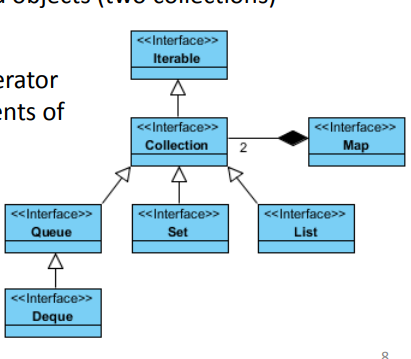
\includegraphics[scale=0.5]{Selection_013.png}
\end{document}
